\subsection*{Modeling scRNA-seq data}
\begin{frame}
  \frametitle{Droplet scRNAseq is not zero-inflated \cite{svensson2020droplet}}
  \begin{itemize}
  \item
    The original "dropout" problem of yielding an inflation of zero values
    in scRNA-seq data was in the description of single-cell differential
    expression (SCDE) \cite{kharchenko2014bayesian}, which was on low-throughput
    plate-based methods, like Smart-seq and STRT-seq.
  \item
    Investigate the number of zeros value using \mywarn{negative control data}
    (like endogenous RNA, ERCC spike-ins) with no
    biological variation. 
  \item
    When scaling the counts by total counts in cells, even a \myemph{Poisson
      distribution} can explain the fraction of zeros well.
  \item
    Heterogeneous cells showed bad fittings, i.e., more zeros than expected.
  \item
    Suggest that additional zero values in biological data are likely due to
    \myemph{biological variation}. 
  \end{itemize}
\end{frame}

\begin{frame}
  \frametitle{Demystifying drop-outs in single-cell UMI data
    \cite{kim2020demystifying}}
  \begin{itemize}
  \item
    They observe that most drop-outs disappear once cell-type heterogeneity is
    resolved. The simple Poisson distribution is then sufficient to fully leverage
    the biological information in the UMI data.
  \item
    Zero proportions are effective measures for cell-type heterogeneity.
  \item
    Sequencing depths are confounded with cell types and size factor-based
    adjustment can obscure biological information.
  \item
    Proposed a zero ratio based t-test to select the zero-inflated genes as cell
    features. 
  \end{itemize}
\end{frame}

% \begin{frame}
%   \frametitle{Multinomial model on scRNASeq \cite{townes2019feature}}
%     Under a multinomial distribution on the observed UMI counts, 74\%-90\%
%     zeros, 22-30\% ones, and less than 4\% values above one. This will
%     artificially enhance the gap between zero and nonzeros values on
%     log-normalized data.
%     \begin{figure}
%       \centering
%       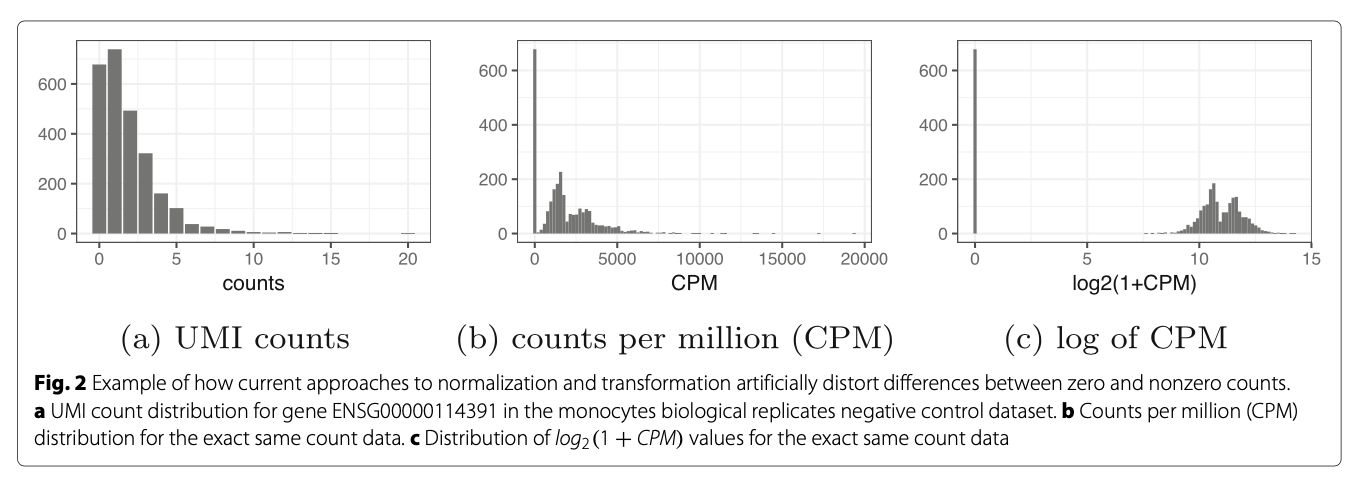
\includegraphics[width=\textwidth]{lognorm_artificial_zeroinflation}
%     \end{figure}
% \end{frame}
